\documentclass[aspectratio=169]{beamer}
\usetheme{Madrid}
\usecolortheme{beaver}
\usepackage[utf8]{inputenc}
\usepackage[T1]{fontenc}
\usepackage{tikz}
\usepackage{amssymb}
\usepackage{graphicx}
\setbeamertemplate{navigation symbols}{}
\setbeamercolor{title}{fg=white,bg=cyan!60!black}
\setbeamercolor{frametitle}{fg=white,bg=cyan!50!black}
\setbeamercolor{block title}{bg=cyan!15,fg=black}
\setbeamercolor{block body}{bg=cyan!5,fg=black}

\title{G7 — Game States}
\subtitle{Menu → playing → paused → game-over → win}
\author{ByteForge --- Grade 7 --- Game Maker --- Week Overview}
\date{}

\begin{document}

\begin{frame}
    \titlepage
\end{frame}

\begin{frame}{This Week's Plan}
    \begin{itemize}
        \item Lesson 1: The State Variable
        \item Lesson 2: Switching States
        \item Lesson 3: Pause Overlay
        \item[$\bigstar$] BOSS --- Full Game Loop w/ Screens (\texttt{lessonBoss.tex})
    \end{itemize}
\end{frame}

\begin{frame}{Real-World Example}
    \Large
    Every app you use has "states": a login screen, a loading spinner, the main screen, an error message — the same menu/playing/paused/gameover idea, just with different names. Minecraft has this too: title screen, world-loading screen, playing, the ESC pause menu, and the respawn/death screen are all states of ONE running program.
\end{frame}


\begin{frame}{Image}
    \begin{center}
    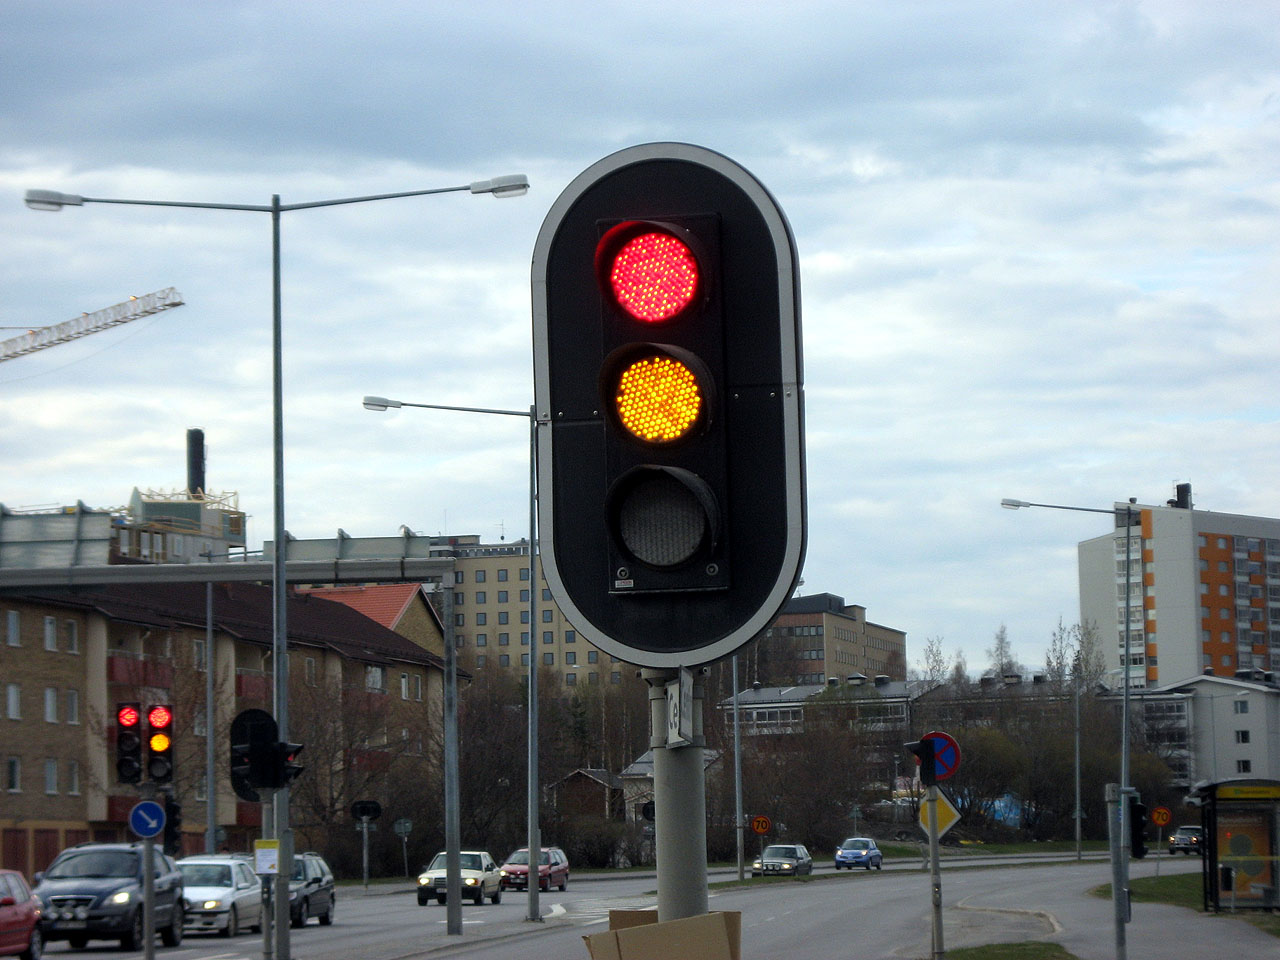
\includegraphics[width=0.55\textwidth]{../images/traffic.jpg}

    \small LED traffic lights, public domain (PD-self), via Wikimedia Commons
    \end{center}
\end{frame}

\begin{frame}{Let Them Discover}
    \Large
    List every distinct "screen" Minecraft (or any game) shows you from opening the app to actually playing (splash screen, menu, loading, playing, pause, death/game over). How many states is that, really?
\end{frame}

\begin{frame}{Files in This Folder}
    \small
    \begin{itemize}
        \item \texttt{lesson1.tex} --- The State Variable
        \item \texttt{lesson2.tex} --- Switching States
        \item \texttt{lesson3.tex} --- Pause Overlay
        \item \texttt{lessonBoss.tex} --- BOSS: Full Game Loop w/ Screens
    \end{itemize}
    \vspace{0.5em}
    \normalsize Each lesson file is its own short deck --- open the one for
    the specific day you're teaching, not this whole overview.
\end{frame}

\end{document}
